\section{Cumin}
\label{sec:cumin}

\begin{spice}\label{spice:cumin}
\textsc{Cumin} \hfill \href{https://powo.science.kew.org/taxon/840882-1}{POWO} \\
\textbf{English:} \textit{cumin}. 
\textbf{Arabic:} {\arabicfont{كمون }} \textit{kammūn}. 
\textbf{Chinese:} {\tradchinesefont{孜然}} \textit{zī​rán}. 
\textbf{Hungarian:} \textit{római kömény} [Roman cumin].  \\
\noindent{\color{black}\rule[0.5ex]{\linewidth}{.5pt}}
\begin{tabular}{@{}p{0.25\linewidth}@{}p{0.75\linewidth}@{}}
Plant species: & \taxonn{Cuminum cyminum}{L.} \\
Family: & \textit{Apiaceae/Umbelliferae} \\
Plant part used: & fruit \\
Region of origin: & W. \& C. Asia; India  \\
Cultivated in: & India, Iran, Lebanon \\
Color: & light brown \\
\end{tabular}
\end{spice}

\begin{figure}[!ht]
	\vspace{-2ex}
	\centering
	\subfloat{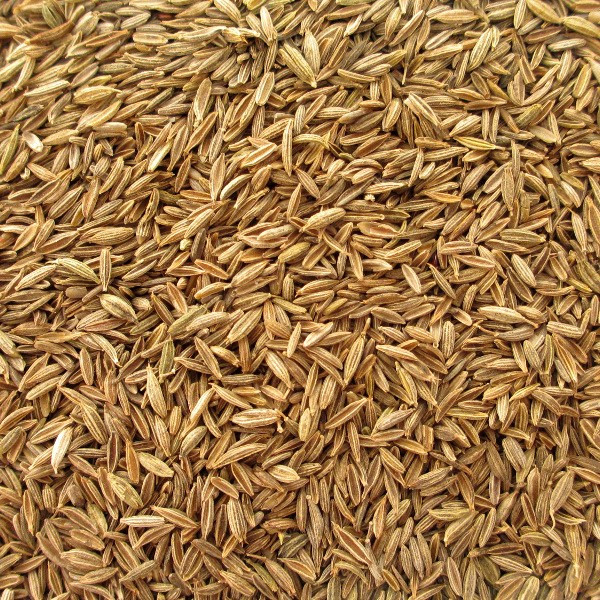
\includegraphics[width=0.3\linewidth]{imgs/spices/cumin-1.jpg}}
	\hfill
	\subfloat{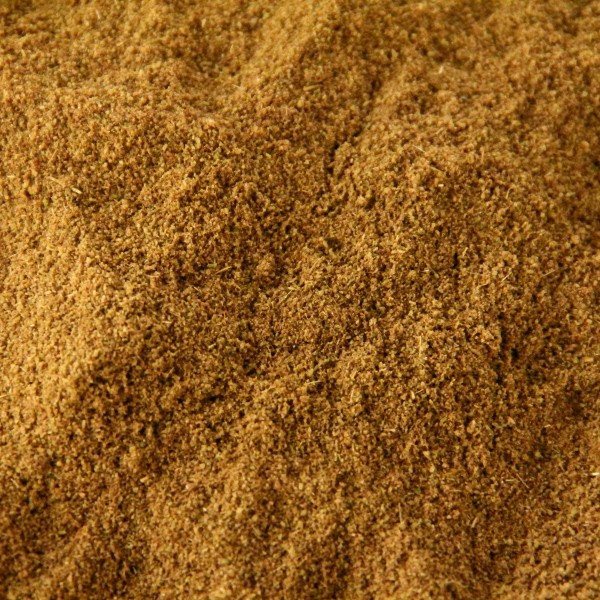
\includegraphics[width=0.3\linewidth]{imgs/spices/cumin-2.jpg}}
% 	\hfill
% 	\subfloat{\includegraphics[width=0.3\linewidth]{imgs/spices/cumin3.jpg}}
	\caption[Cumin]{ (\taxon{Cuminum cyminum}). Credit: Aromatiques.}
	\label{fig:cumin_imgs}
\end{figure}

\subsection{The Botany of Cumin}

\subsection{The History of Cumin}

\subsection{The Names of Cumin}

\subsubsection{English}

\begin{etymology}\label{ety:cumin}
English \textit{cumin}, Middle English cumin, comin was either from French (like Middle Dutch comijn, Dutch komijn), or altered from Old English cymen after French. (Old English \textit{cymen}); cf. cognates Old High German chumin, cumin, also chumil (Middle High German kümel, German kümmel), Swedish kummin, Danish kummen. The word has also come down in the Romanic languages, Italian cumino, comino, Spanish comino, Portuguese cominho, Old French cumin, comin. 
< Latin \textit{cumīnum} `id.'
< Ancient Greek {κύμῑνον} \textit{kúmīnon} `id.', The Greek κύμῑνον is supposed to have been a foreign word, cognate in origin with the Semitic names
< Semitic \textit{*kmn} `id.'; cf. cognates Arabic \textit{kammūn}; Hebrew \textit{kammōn}; Akkadian \textit{kamūnu}\footnote{\textcite[s.v. cumin]{oed}; }
\end{etymology}

\begin{table}[!ht]
\centering
\begin{tabularx}{\textwidth}{@{}l>{\itshape \small}lL>{\small}l@{}}
\toprule
\textbf{\#} & \multicolumn{1}{l}{\textbf{Species}} & \multicolumn{1}{l}{\textbf{Name}} & \multicolumn{1}{l}{\textbf{Source}} \\
\midrule
\textbf{1}	& \textbf{Cuminum cyminum}	& \textbf{cumin}	& \textbf{\textcite{van_wyk_culinary_2014}} \\
2	& Cuminum cyminum	& cumin seed	& \textcite{van_wyk_culinary_2014} \\
\bottomrule
\end{tabularx}
\caption{Various names for cumin in English.}
\label{table:names_cumin_en}
\end{table}



\subsubsection{Arabic}

\begin{etymology}\label{ety:kammun}
\textbf{Arabic} {كمون} \textit{kammūn} `cumin'
< \textbf{Aramaic} {\he{כַּמֹּונָֹא}/\sy{ܩܰܡܽܘܢܳܐ}} \textit{kammōnā} `cumin'; cf. cognates Old Armenian \hy{չաման} \textit{čʿaman}
< \textbf{Akkadian} {\cu{𒌑𒁷𒊺𒉪} Ú.GAMUN} \textit{kamūnu} `cumin'\footnote{}
\end{etymology}

\begin{table}[!ht]
    \caption{Various names for cumin in Arabic.}
\centering
\begin{tabularx}{\textwidth}{@{}l>{\itshape \small}lr>{\itshape}lL>{\small}l@{}}
\toprule
\textbf{\#} & \multicolumn{1}{l}{\textbf{Species}} & \multicolumn{1}{l}{\textbf{Name}} & \multicolumn{1}{l}{\textbf{Tr.}} & \multicolumn{1}{l}{\textbf{Gloss}} & \multicolumn{1}{l}{\textbf{Source}} \\
\midrule
\textbf{1}	& \textbf{Cuminum cyminum}	& \textbf{كمون }	& \textbf{kammūn}	& \textbf{}	& \textbf{\textcite{wehr_dictionary_1976}} \\
2	& Cuminum cyminum	& سنوت	& sannūt	& 	& \textcite{lane_arabic-english_1863} \\
\bottomrule
\end{tabularx}
\label{table:names_cumin_ar}
\end{table}



\subsubsection{Chinese}

\begin{etymology}\label{ety:ziran}
\textbf{Mandarin Chinese} \tc{孜然} \textit{zī​rán} `cumin', modern loan from Uyghur (the historic term is \tc{蒔蘿} from Middle Persian \textit{*zīra} during Tang dynasty)
< \textbf{Uyghur} {زىرە} \textit{zirä} `cumin'
< \textbf{Persian} {زیره} \textit{zīra} `cumin', distantly related to Sanskrit \textit{jīraka} (zire-ye siyāh [black cumin] `caraway'; zire-ye sabz [green cumin] `cumin'); cf. cognates Sogdian zyr'kk /zîrê/; Hindi-Urdu \textit{zīrā}
<\textss{?} \textbf{Sanskrit} {जीर} \textit{jīra} `cumin'; cf. Hindi जीरा \textit{jīrā}; English \textit{jeera}\footnote{\textcites[383]{laufer_sino-iranica_1919}[45]{sulaiman_uyghur_2020}[]{liu_hanyu_1985}; \textcite[561]{schwarz_uyghur-english_1992}; \textcite[634]{steingass_comprehensive_1892}; \textcites[375]{mcgregor_oxford_1993}}
\end{etymology}

\begin{table}[!ht]
\centering
\begin{tabularx}{\textwidth}{@{}l>{\itshape \small}ll>{\itshape}lL>{\small}l@{}}
\toprule
\textbf{\#} & \multicolumn{1}{l}{\textbf{Species}} & \multicolumn{1}{l}{\textbf{Name}} & \multicolumn{1}{l}{\textbf{Tr.}} & \multicolumn{1}{l}{\textbf{Gloss}} & \multicolumn{1}{l}{\textbf{Source}} \\
\midrule
1	& Cuminum cyminum	& \tradchinesefont{茴香籽}	& huíxiāngzǐ	& hui-spice-seed	& \textcite{mdbg} \\
2	& Cuminum cyminum	& \tradchinesefont{枯茗}	& kūmíng	& withered-tea	& \textcite{mdbg} \\
3	& Cuminum cyminum	& \tradchinesefont{羅馬葛縷子}	& luómǎ gě​lǚ​zi	& Roman-caraway	&  \\
4	& Cuminum cyminum	& \tradchinesefont{馬芹子}	& mǎqínzi	& horse-celery-seed	&  \\
5	& Cuminum cyminum	& \tradchinesefont{蒔蘿}	& shíluó	& dill-turnip	& \textcite{laufer_sino-iranica_1919} \\
6	& Cuminum cyminum	& \tradchinesefont{小茴香}	& xiǎohuíxiāng	& small-hui-spice-seed	& \textcite{laufer_sino-iranica_1919} \\
\textbf{7}	& \textbf{Cuminum cyminum}	& \textbf{\tradchinesefont{孜然}}	& \textbf{zīrán}	& \textbf{}	& \textbf{\textcite{mdbg}} \\
8	& Cuminum cyminum	& \tradchinesefont{孜然芹}	& zī​ránqín	& cumin-celery	& \textcite{hu_food_2005} \\
9	& Cuminum cyminum	& \tradchinesefont{阿拉伯茴香}	& ālābó huíxiāng	& Arabian fennel	& \textcite{mdbg} \\
10	& Cuminum cyminum	& \tradchinesefont{安息茴香}	& ānxī huíxiāng	& Parthian fennel	& \textcite{mdbg} \\
11	& Cuminum cyminum	& \tradchinesefont{歐蒔蘿}	& ōu​ shí​luó	& European dill	& \textcite{mdbg} \\
\bottomrule
\end{tabularx}
\caption{Various names for cumin in Chinese.}
\label{table:names_cumin_zh}
\end{table}



\subsubsection{Summary}

\begin{table}[!ht]
\centering
\begin{tabularx}{\textwidth}{@{}ll>{\itshape}lLl>{\small}l@{}}
\toprule
\textbf{\#} & \textbf{Language} & \multicolumn{1}{l}{\textbf{Term}} & \textbf{Gloss} & \textbf{Loan} & \multicolumn{1}{l}{\textbf{Source}} \\
\midrule
1	& English	& cumin	& 	& yes	& \textcite{oed} \\
2	& English	& cumin seed	& 	& no	& \textcite{oed} \\
\midrule
1	& Arabic	& kammūn	& 	& yes	& \textcite{wehr_dictionary_1976} \\
\midrule
1	& Chinese	& huíxiāngzǐ	& hui-spice-seed	& no	& \textcite{mdbg} \\
2	& Chinese	& kūmíng	& withered-tea	& yes	& \textcite{mdbg} \\
3	& Chinese	& shíluó	& dill-turnip	& yes	& \textcite{kleeman_oxford_2010} \\
4	& Chinese	& zīrán	& 	& yes	& \textcite{mdbg} \\
5	& Chinese	& zī​ránqín	& cumin-celery	& no	& \textcite{mdbg} \\
6	& Chinese	& ālābó huíxiāng	& Arabian fennel	& no	& \textcite{mdbg} \\
7	& Chinese	& ānxī huíxiāng	& Parthian fennel	& no	& \textcite{mdbg} \\
8	& Chinese	& ōu​ shí​luó	& European dill	& no	& \textcite{mdbg} \\
\bottomrule
\end{tabularx}
\caption{Conventionalized names for cumin in English, Arabic, and Chinese, found in dictionaries.}
\label{table:names_cumin}
\end{table}




























% EE:
% cum(m)in 
% XII. — OF. cumin, comin :- L. cumīnum — Gr. kúmīnon, prob. of Sem. orig.

% OE:
% cumin (n.)
% "fennel-like umbelliferous plant of the carrot family found wild in Egypt and Syria and cultivated for its fruit," Old English cymen, from Latin cuminum, from Greek kyminon, cognate with Hebrew kammon, Arabic kammun. Related: Cumic.

% MW:
% Middle English comin, cummin, from Old English cymen; akin to Old High German kumīn cumin, Middle Low German kömen, all from a prehistoric West Germanic word borrowed from Latin cuminum, from Greek kyminon, of Semitic origin; akin to Arabic kammūn cumin, Hebrew kammōn
% First Known Use: before 12th century

% AH:
% [Middle English, from Old French, from Latin cumīnum, from Greek kumīnon, probably of Semitic origin; see kmn in Semitic roots.]

% WK: 
% From Middle English comyn, from Old English cymen (which is cognate with Old High German kumin) and Old French cummin, both from Latin cuminum, from Ancient Greek κύμινον (kúminon), a Semitic borrowing ultimately to be traced to Akkadian (Ú.GAMUN /kamūnu/, “cumin”).[1][2][3]. Possibly related to caraway. 



